% =============================================================================
% DSP501 Final Report — Environmental Sound Classification
% LaTeX IEEE Conference Format
% =============================================================================
\documentclass[conference]{IEEEtran}

% === Packages ===
\usepackage[utf8]{inputenc}
\usepackage[T1]{fontenc}
\usepackage{amsmath,amssymb,amsfonts}
\usepackage{graphicx}
\usepackage{booktabs}
\usepackage{multirow}
\usepackage{array}
\usepackage{xcolor}
\usepackage{hyperref}
\usepackage{cleveref}
\usepackage{float}
\usepackage{subcaption}
\usepackage{algorithm}
\usepackage{algpseudocode}
\usepackage{cite}
\usepackage{balance}
\usepackage{url}
\usepackage{siunitx}
\usepackage{tabularx}

% === Graphics path ===
\graphicspath{{../results/figures/}}

% === Hyperref setup ===
\hypersetup{
    colorlinks=true,
    linkcolor=blue!70!black,
    citecolor=green!50!black,
    urlcolor=blue!70!black
}

% === Custom commands ===
\newcommand{\pipeA}{\textbf{Pipeline~A}}
\newcommand{\pipeB}{\textbf{Pipeline~B}}
\newcommand{\US}{UrbanSound8K}

% =============================================================================
\begin{document}

\title{Does DSP Preprocessing Improve AI-Based\\Environmental Sound Classification?}

\author{
\IEEEauthorblockN{DSP501 --- Digital Signal Processing Final Project}
\IEEEauthorblockA{March 2026\\
Dataset: UrbanSound8K (Salamon et al., 2014)}
}

\maketitle

% =============================================================================
\begin{abstract}
This project investigates whether traditional DSP preprocessing improves AI-based environmental sound classification. We design and compare two pipelines on the \US{} dataset (8,732 clips, 10 classes): \pipeA{} feeds raw audio directly to classifiers, while \pipeB{} applies FIR bandpass filtering, pre-emphasis, and amplitude normalization before classification. Three models are evaluated---SVM, Random Forest, and CNN-2D---using 10-fold cross-validation with predefined folds. Results show \textbf{no statistically significant difference} between the two pipelines (all $p > 0.05$, all $|d| < 0.2$), suggesting that modern feature extraction methods (MFCCs, mel spectrograms) already capture the relevant information, making explicit DSP preprocessing redundant for this task.
\end{abstract}

\begin{IEEEkeywords}
Environmental Sound Classification, Digital Signal Processing, FIR Filter, MFCC, Mel Spectrogram, SVM, Random Forest, CNN, UrbanSound8K
\end{IEEEkeywords}

% =============================================================================
\section{Introduction}
\label{sec:intro}

% -----------------------------------------------------------------------------
\subsection{Motivation}

Environmental Sound Classification (ESC) is a fundamental problem in audio signal processing with applications in smart cities, surveillance, wildlife monitoring, and assistive technologies~\cite{salamon2014}. A key question in the field is whether traditional DSP preprocessing---filtering, pre-emphasis, normalization---provides meaningful improvements when combined with modern machine learning methods.

% -----------------------------------------------------------------------------
\subsection{Research Question}

\begin{quote}
\textit{Does applying classical DSP preprocessing (bandpass filtering, pre-emphasis, normalization) to audio signals improve the accuracy of environmental sound classification compared to using raw audio directly?}
\end{quote}

% -----------------------------------------------------------------------------
\subsection{Approach}

We design two experimental pipelines:
\begin{itemize}
    \item \pipeA{} (Baseline): Raw audio $\rightarrow$ Feature Extraction $\rightarrow$ Classification
    \item \pipeB{} (DSP-Enhanced): Raw audio $\rightarrow$ FIR Bandpass $\rightarrow$ Pre-emphasis $\rightarrow$ Normalization $\rightarrow$ Feature Extraction $\rightarrow$ Classification
\end{itemize}

Both pipelines are evaluated with identical models and evaluation methodology, differing only in whether DSP preprocessing is applied. Three classifiers are tested: SVM, Random Forest, and CNN-2D.

% =============================================================================
\section{Dataset}
\label{sec:dataset}

% -----------------------------------------------------------------------------
\subsection{UrbanSound8K}

The \US{} dataset~\cite{salamon2014} contains 8,732 labeled sound excerpts ($\leq 4$~seconds) of urban sounds across 10 classes. \Cref{tab:dataset} summarizes the class distribution.

\begin{table}[htbp]
\centering
\caption{UrbanSound8K class distribution and signal characteristics.}
\label{tab:dataset}
\begin{tabular}{@{}lrl@{}}
\toprule
\textbf{Class} & \textbf{Samples} & \textbf{Category} \\
\midrule
air\_conditioner   & 1,000 & Stationary \\
car\_horn          & 429   & Non-stationary \\
children\_playing  & 1,000 & Stationary-like \\
dog\_bark          & 1,000 & Non-stationary \\
drilling           & 1,000 & Non-stationary \\
engine\_idling     & 1,000 & Stationary \\
gun\_shot          & 374   & Non-stationary \\
jackhammer         & 1,000 & Stationary-like \\
siren              & 929   & Stationary-like \\
street\_music      & 1,000 & Stationary-like \\
\midrule
\textbf{Total}     & \textbf{8,732} & \\
\bottomrule
\end{tabular}
\end{table}

Key properties:
\begin{itemize}
    \item 10 predefined folds for cross-validation (never shuffled)
    \item Class imbalance: \textit{car\_horn} (429) and \textit{gun\_shot} (374) are underrepresented
    \item All audio resampled to \textbf{22,050~Hz}, padded/truncated to \textbf{4~seconds} (88,200 samples)
\end{itemize}

% -----------------------------------------------------------------------------
\subsection{Signal Characteristics}

Stationarity analysis reveals two distinct signal groups:
\begin{itemize}
    \item \textbf{Stationary-like}: relatively stable spectral content (air\_conditioner, engine\_idling, children\_playing, jackhammer, siren, street\_music)
    \item \textbf{Non-stationary}: impulsive/transient characteristics (car\_horn, dog\_bark, gun\_shot, drilling)
\end{itemize}

Spectral analysis further groups classes by dominant frequency bands:
\begin{itemize}
    \item \textbf{Low frequency} ($< 250$~Hz): engine\_idling (64.1\%), air\_conditioner (55.6\%)
    \item \textbf{Mid frequency} (250--1,000~Hz): dog\_bark (60.5\%), car\_horn (45.8\%)
    \item \textbf{High frequency} (1--4~kHz): children\_playing (41.4\%), siren (40.9\%)
    \item \textbf{Broadband}: drilling, jackhammer, gun\_shot
\end{itemize}

\begin{figure}[htbp]
    \centering
    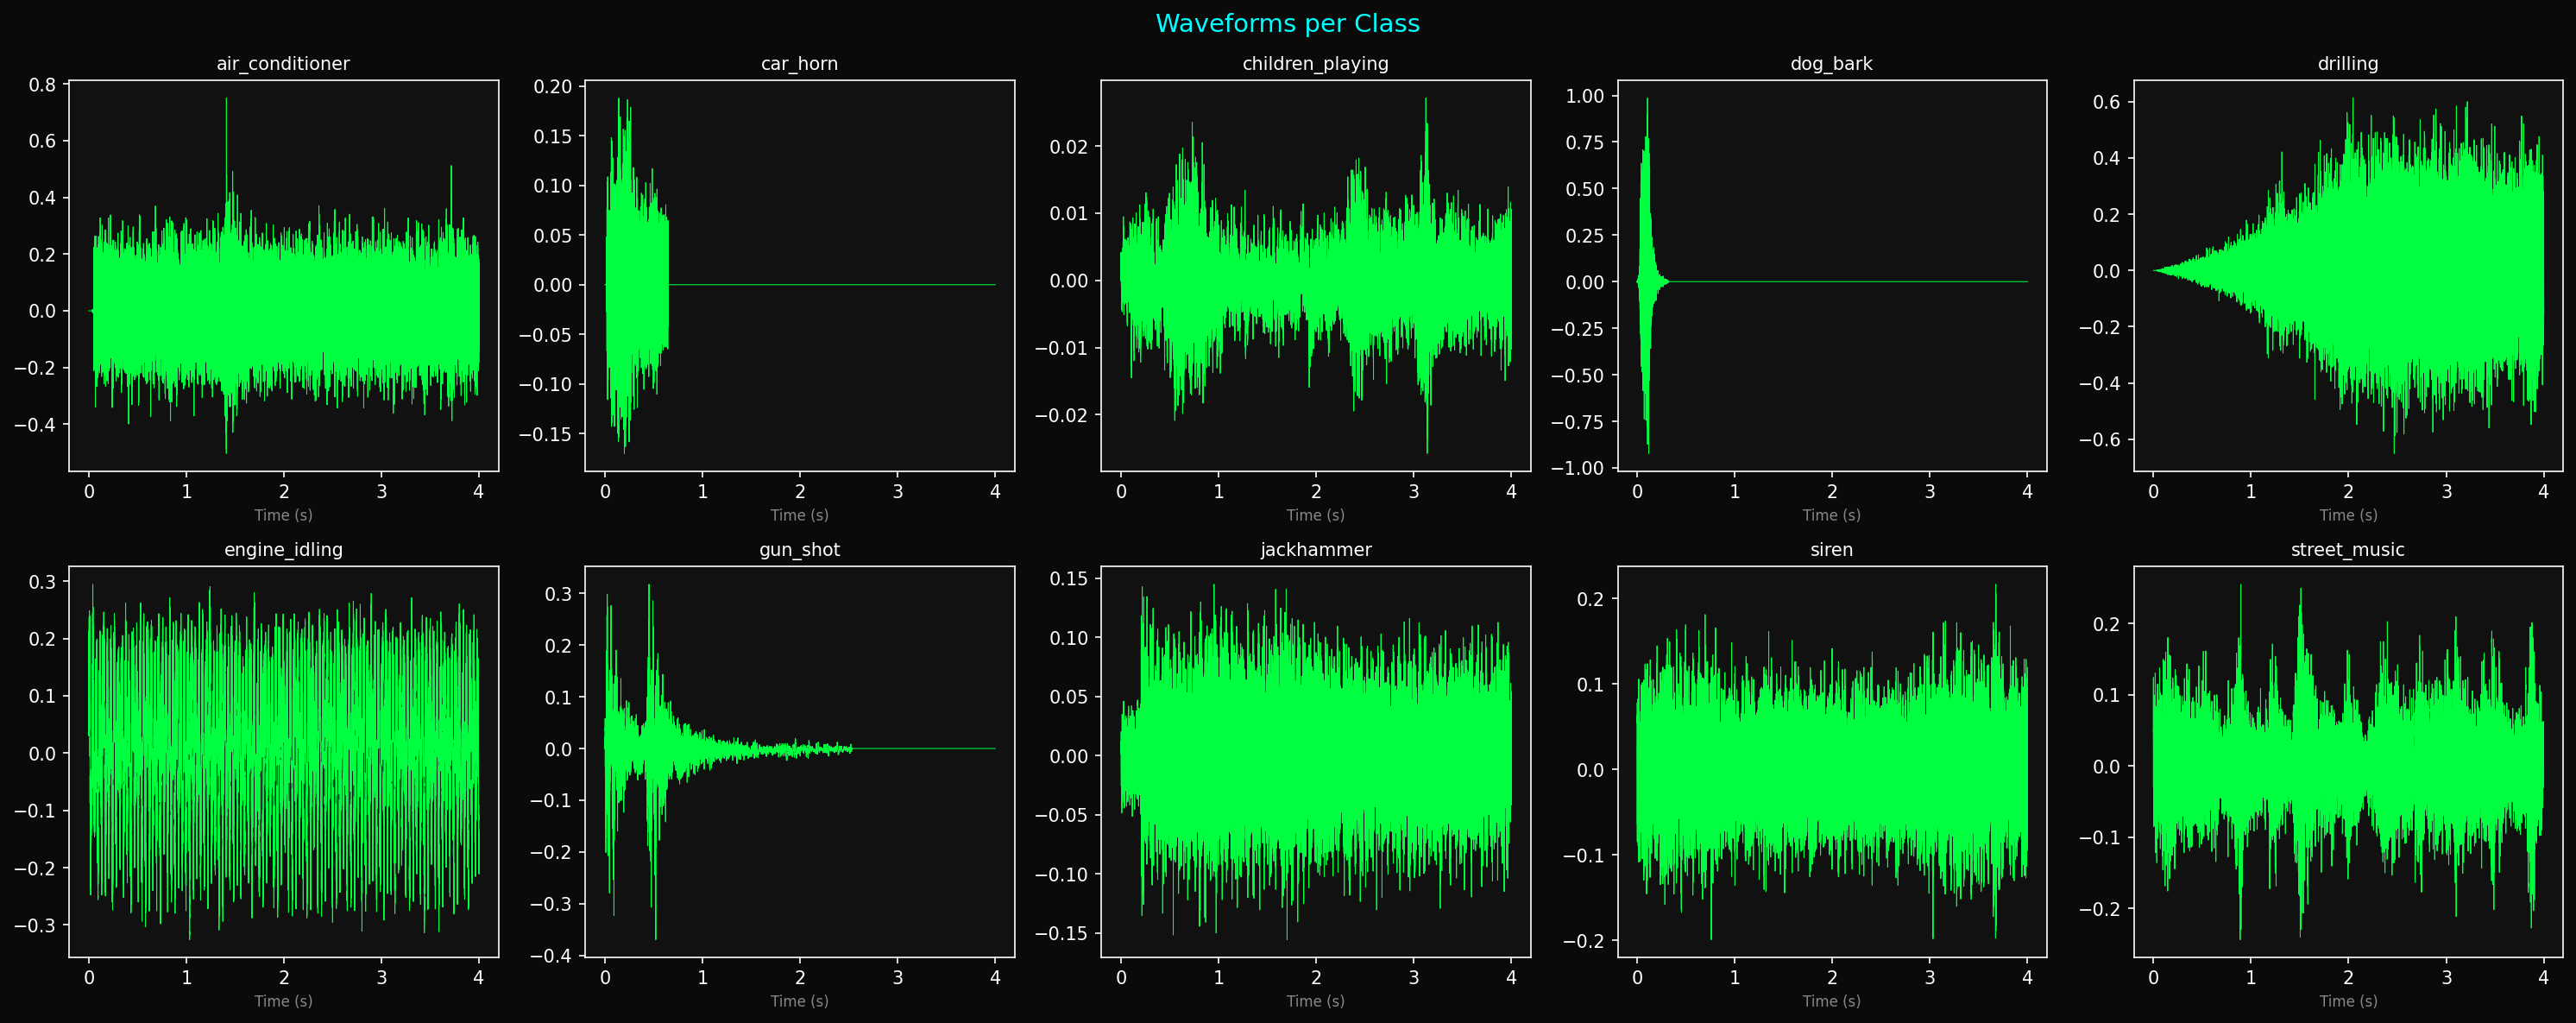
\includegraphics[width=\columnwidth]{fig_waveforms_per_class.png}
    \caption{Raw waveforms for all 10 classes in UrbanSound8K.}
    \label{fig:waveforms}
\end{figure}

\begin{figure}[htbp]
    \centering
    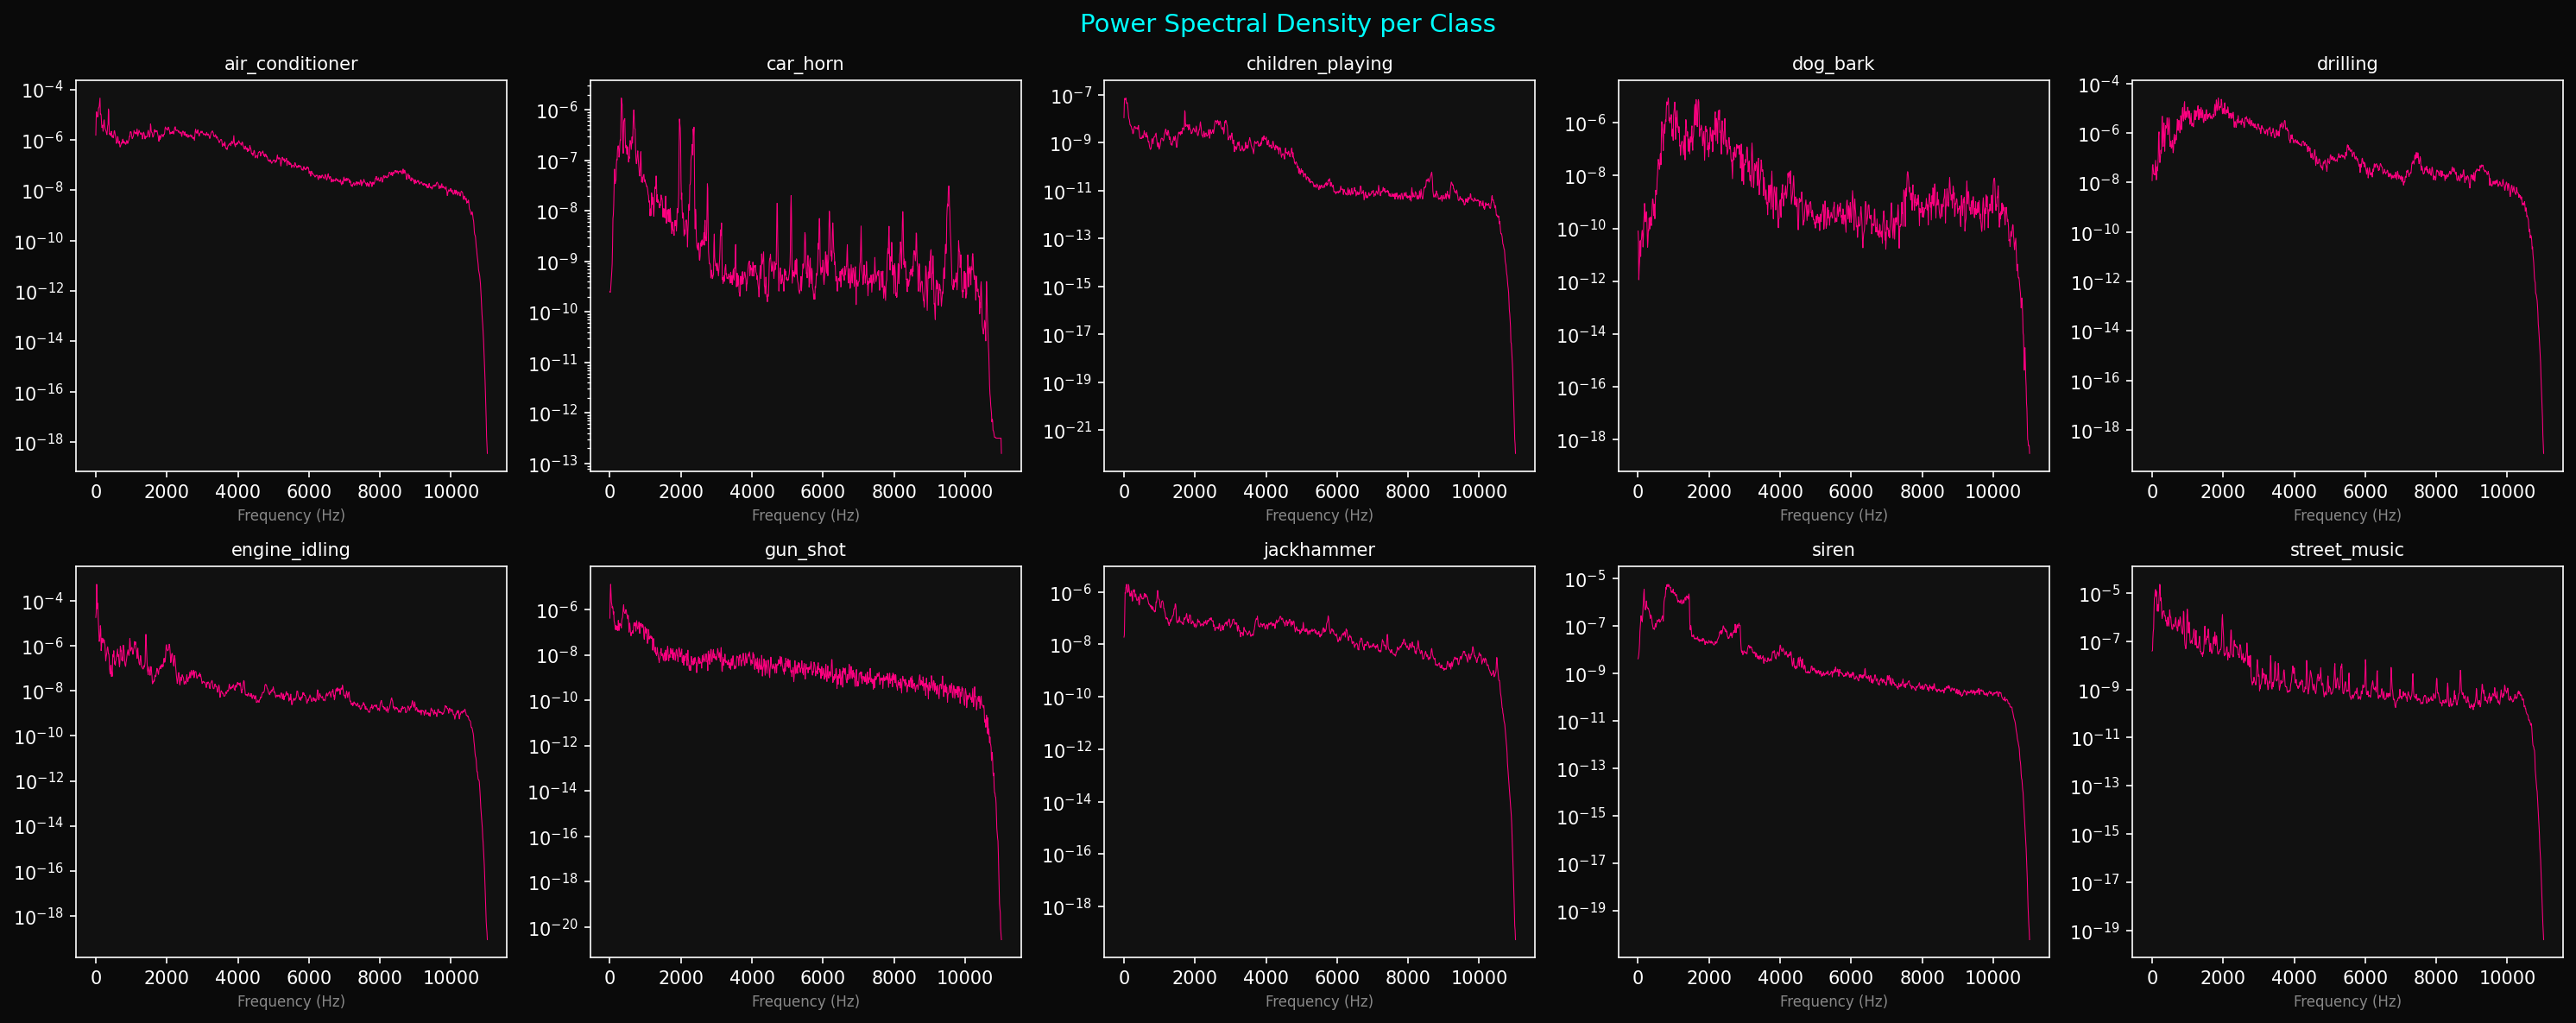
\includegraphics[width=\columnwidth]{fig_psd_per_class.png}
    \caption{Power spectral density (PSD) per class, showing distinct frequency profiles.}
    \label{fig:psd}
\end{figure}

% =============================================================================
\section{DSP Pipeline Design}
\label{sec:dsp}

\pipeB{} applies three sequential DSP stages before feature extraction, as illustrated in \Cref{fig:pipeline}.

\begin{figure}[htbp]
\centering
\fbox{\parbox{0.9\columnwidth}{\centering
\small
$x[n] \xrightarrow{\text{FIR Bandpass}} x_f[n] \xrightarrow{\text{Pre-emphasis}} x_p[n] \xrightarrow{\text{Normalize}} x_{\text{out}}[n]$
}}
\caption{Pipeline~B processing chain.}
\label{fig:pipeline}
\end{figure}

% -----------------------------------------------------------------------------
\subsection{FIR Bandpass Filter}

The FIR bandpass filter is designed using the \textbf{window method} with a Hann window. The ideal bandpass impulse response is:
\begin{equation}
    h_d[n] = \frac{\sin(\omega_h n)}{\pi n} - \frac{\sin(\omega_l n)}{\pi n}
    \label{eq:fir_ideal}
\end{equation}
where $\omega_l = 2\pi \cdot 50 / 22050$ and $\omega_h = 2\pi \cdot 10000 / 22050$.

\textbf{Parameters:}
\begin{itemize}
    \item Passband: 50~Hz -- 10,000~Hz
    \item Order: 101 taps
    \item Window: Hann
    \item Implementation: zero-phase filtering via \texttt{scipy.signal.filtfilt}
\end{itemize}

\textbf{Key properties:}
\begin{itemize}
    \item \textit{Linear phase}: $\phi(\omega) = -\frac{M-1}{2}\omega$, preserving temporal structure
    \item \textit{Constant group delay}: $\tau_g = 50$ samples
    \item \textit{Always stable}: FIR systems have all poles at origin
\end{itemize}

The transfer function is:
\begin{equation}
    H(z) = \sum_{k=0}^{100} h[k] \, z^{-k}
    \label{eq:fir_tf}
\end{equation}

Zero-phase implementation applies forward-backward filtering:
\begin{equation}
    y[n] = \mathcal{F}^{-1}\left\{ |H(e^{j\omega})|^2 \cdot X(e^{j\omega}) \right\}
    \label{eq:zerophase}
\end{equation}

\begin{figure}[htbp]
    \centering
    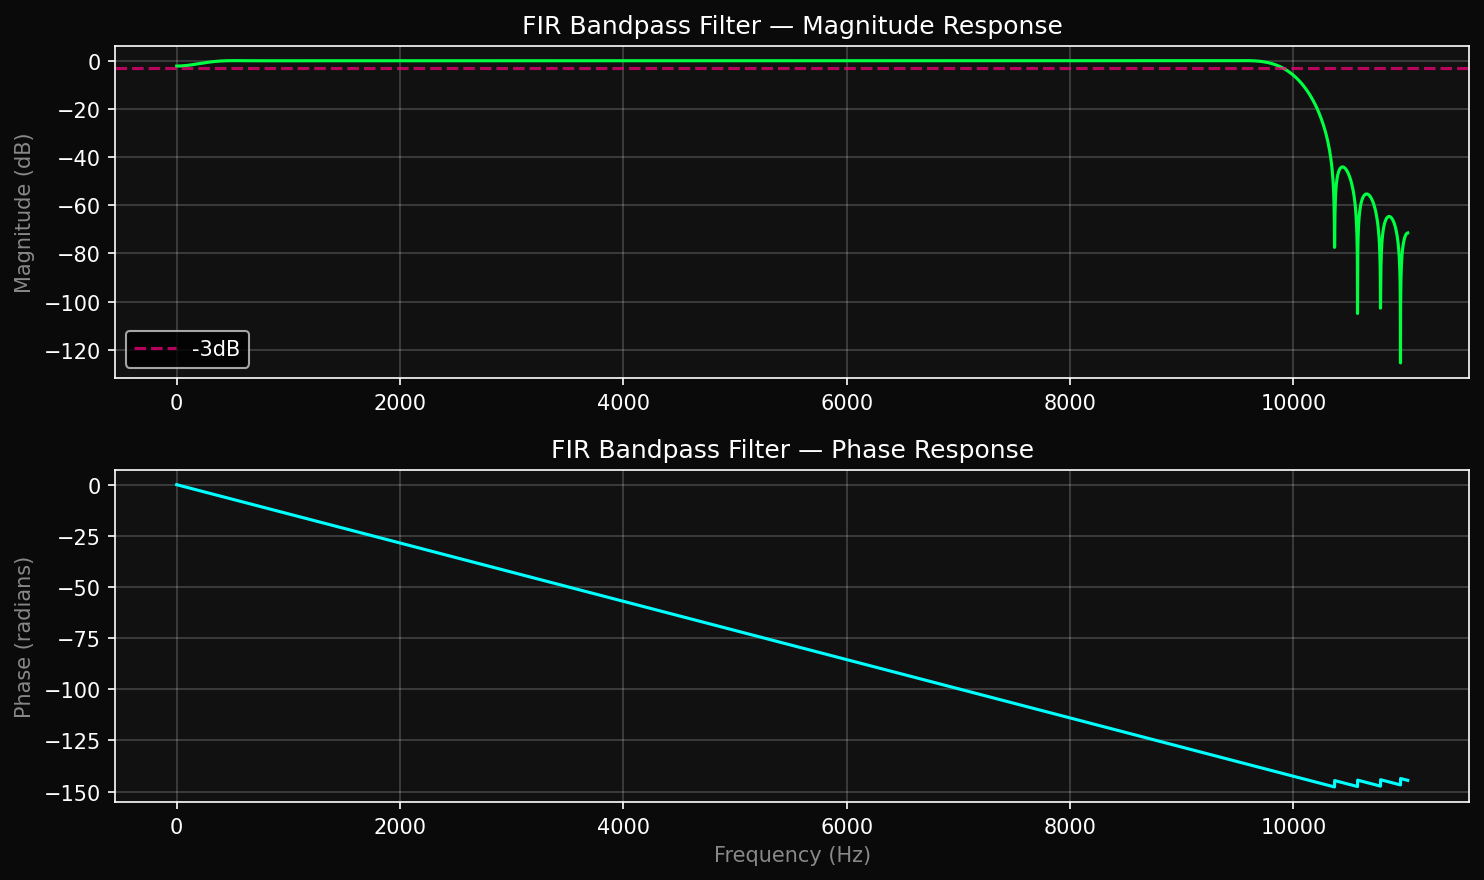
\includegraphics[width=\columnwidth]{fig_fir_frequency_response.png}
    \caption{FIR bandpass filter frequency response: magnitude and phase.}
    \label{fig:fir_response}
\end{figure}

% -----------------------------------------------------------------------------
\subsection{IIR Butterworth Filter (Comparison)}

For comparison, a 5th-order IIR Butterworth bandpass filter was implemented:
\begin{equation}
    |H_a(j\Omega)|^2 = \frac{1}{1 + \left(\frac{\Omega}{\Omega_c}\right)^{2N}}
    \label{eq:iir_butterworth}
\end{equation}

Converted to the digital domain via bilinear transform with frequency pre-warping. The IIR filter is \textbf{stable} (all poles inside the unit circle, verified in \Cref{fig:pole_zero}) but has \textbf{nonlinear phase}, which distorts temporal structure.

\textbf{Decision}: FIR chosen as the primary filter because linear phase is critical for preserving temporal characteristics of environmental sounds.

\begin{figure}[htbp]
    \centering
    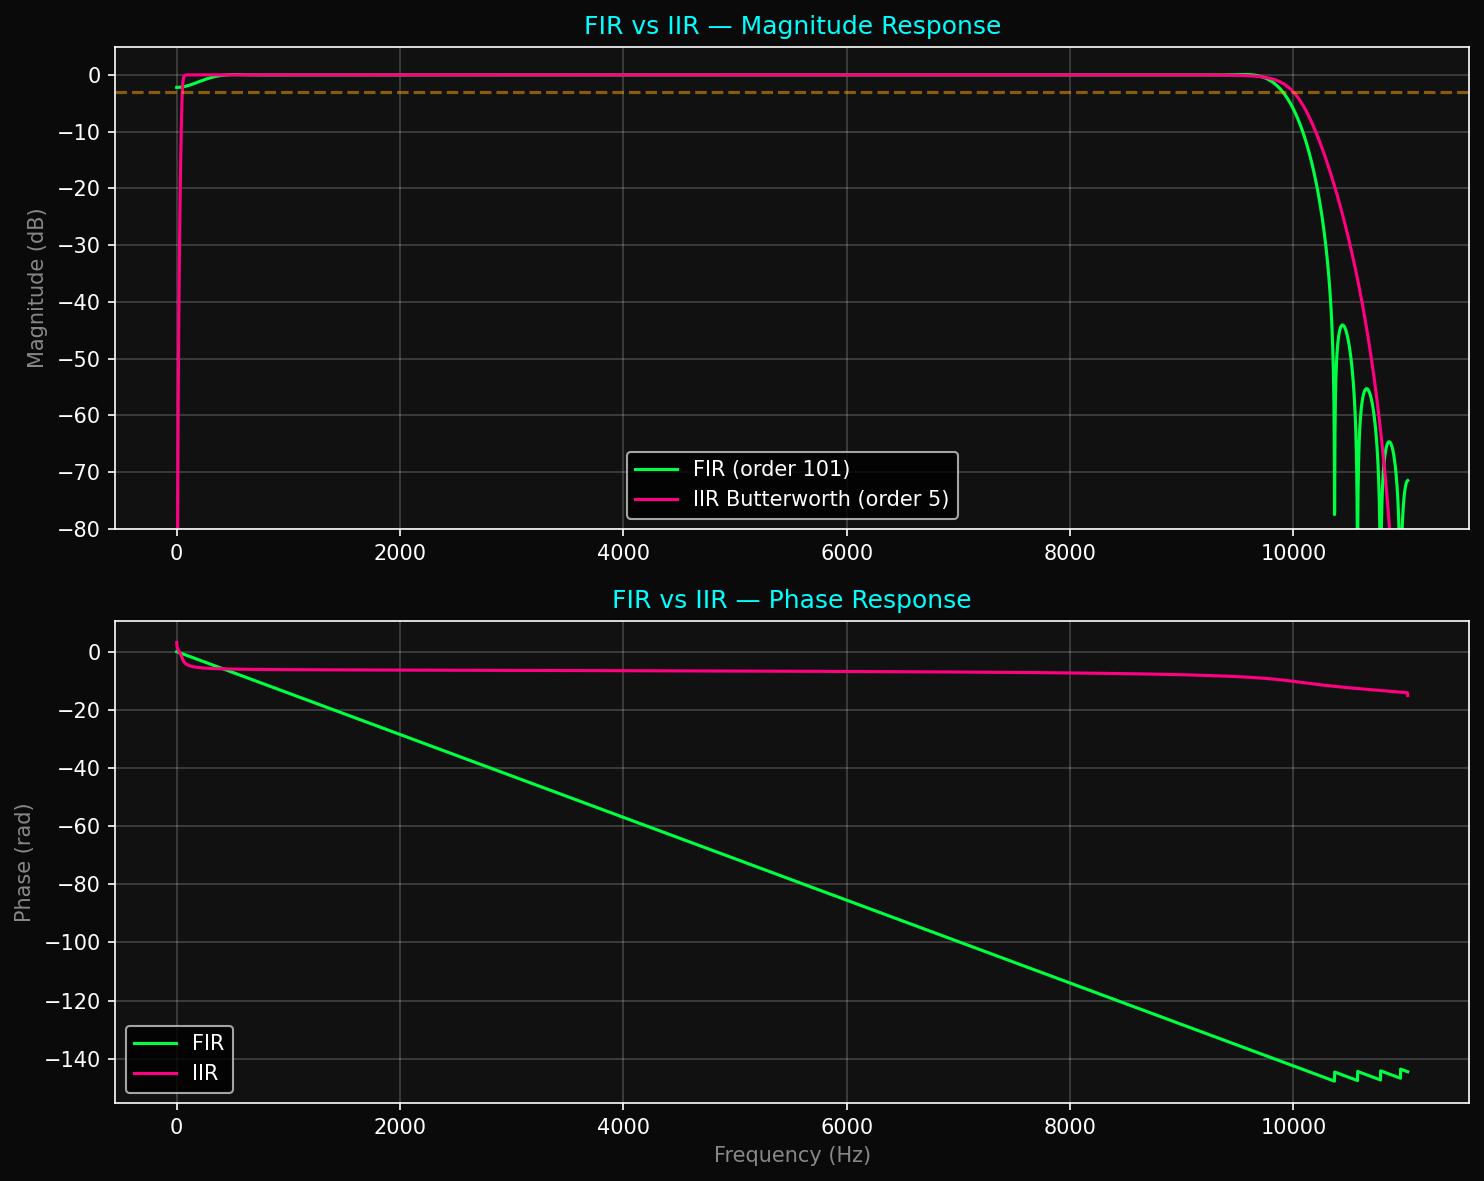
\includegraphics[width=\columnwidth]{fig_fir_vs_iir_comparison.png}
    \caption{FIR vs.\ IIR frequency response comparison.}
    \label{fig:fir_vs_iir}
\end{figure}

\begin{figure}[htbp]
    \centering
    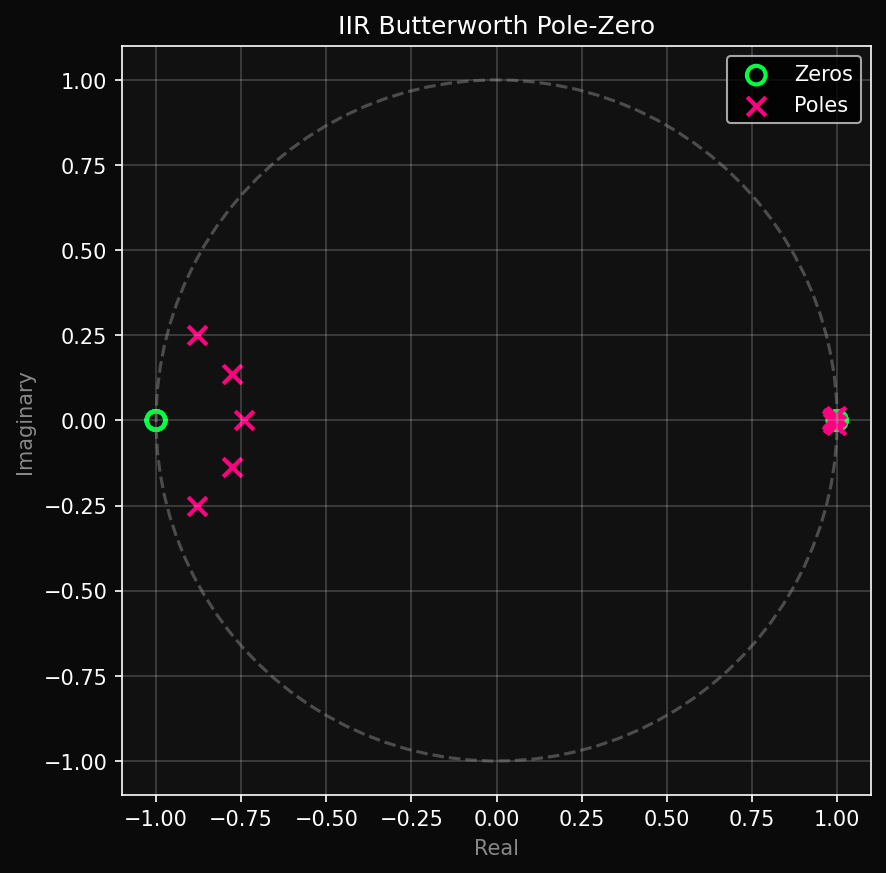
\includegraphics[width=\columnwidth]{fig_iir_pole_zero.png}
    \caption{IIR Butterworth pole-zero diagram. All poles lie inside the unit circle, confirming BIBO stability.}
    \label{fig:pole_zero}
\end{figure}

% -----------------------------------------------------------------------------
\subsection{Pre-emphasis Filter}

A first-order high-pass filter boosts high frequencies:
\begin{equation}
    x_p[n] = x[n] - \alpha \cdot x[n-1], \quad \alpha = 0.97
    \label{eq:preemphasis}
\end{equation}
with transfer function $H_{\text{pre}}(z) = 1 - 0.97z^{-1}$.

% -----------------------------------------------------------------------------
\subsection{Peak Normalization}

Amplitude is scaled to the $[-1, 1]$ range:
\begin{equation}
    x_{\text{out}}[n] = \frac{x_p[n]}{\max_n |x_p[n]|}
    \label{eq:normalize}
\end{equation}

% -----------------------------------------------------------------------------
\subsection{DSP Impact on Signal Quality}

SNR measurements show DSP preprocessing does improve raw signal quality:
\begin{itemize}
    \item \textit{children\_playing}: $+4.5$~dB
    \item \textit{jackhammer}: $+2.9$~dB
    \item Impulsive signals (\textit{car\_horn}, \textit{gun\_shot}): SNR estimation unreliable due to no quiet frames
\end{itemize}

\begin{figure}[htbp]
    \centering
    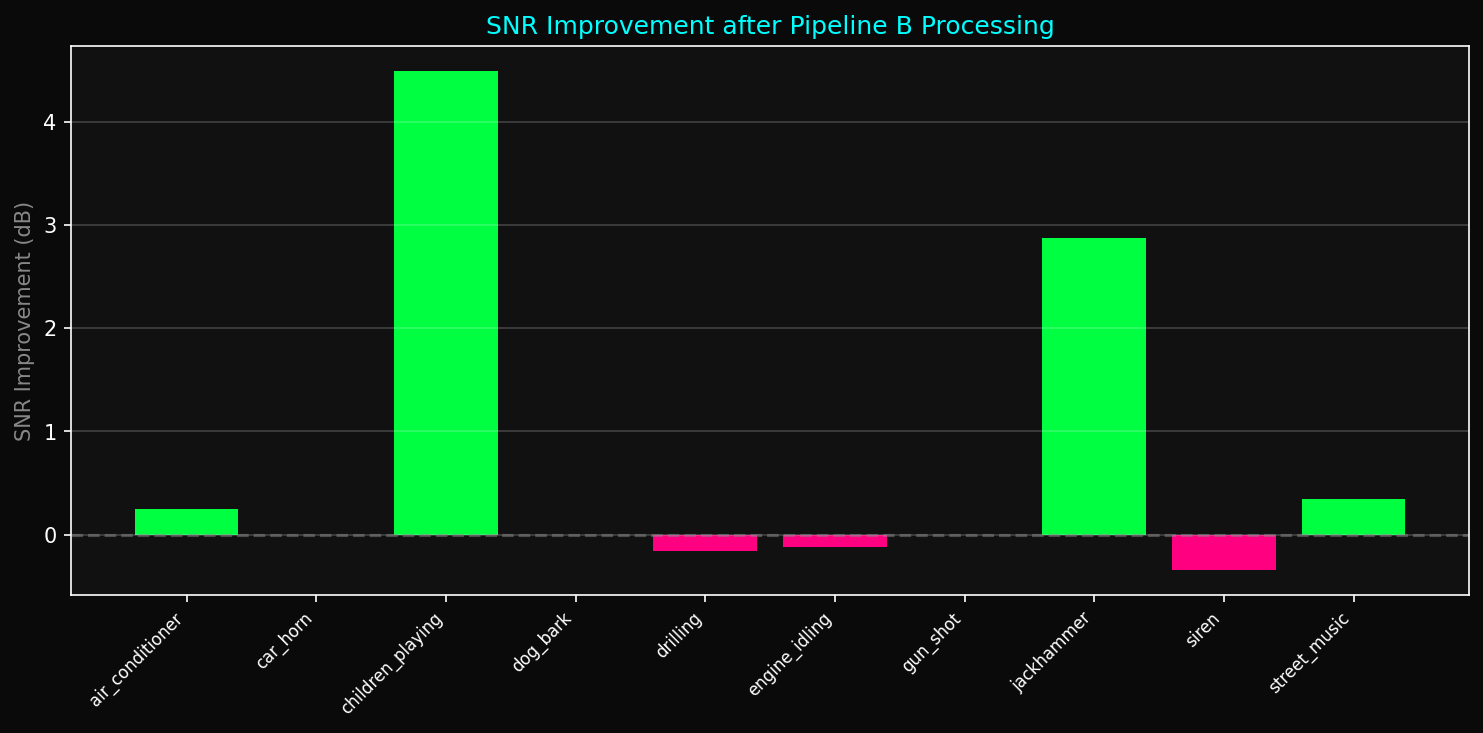
\includegraphics[width=\columnwidth]{fig_snr_improvement.png}
    \caption{SNR improvement from DSP preprocessing per class.}
    \label{fig:snr}
\end{figure}

\begin{figure}[htbp]
    \centering
    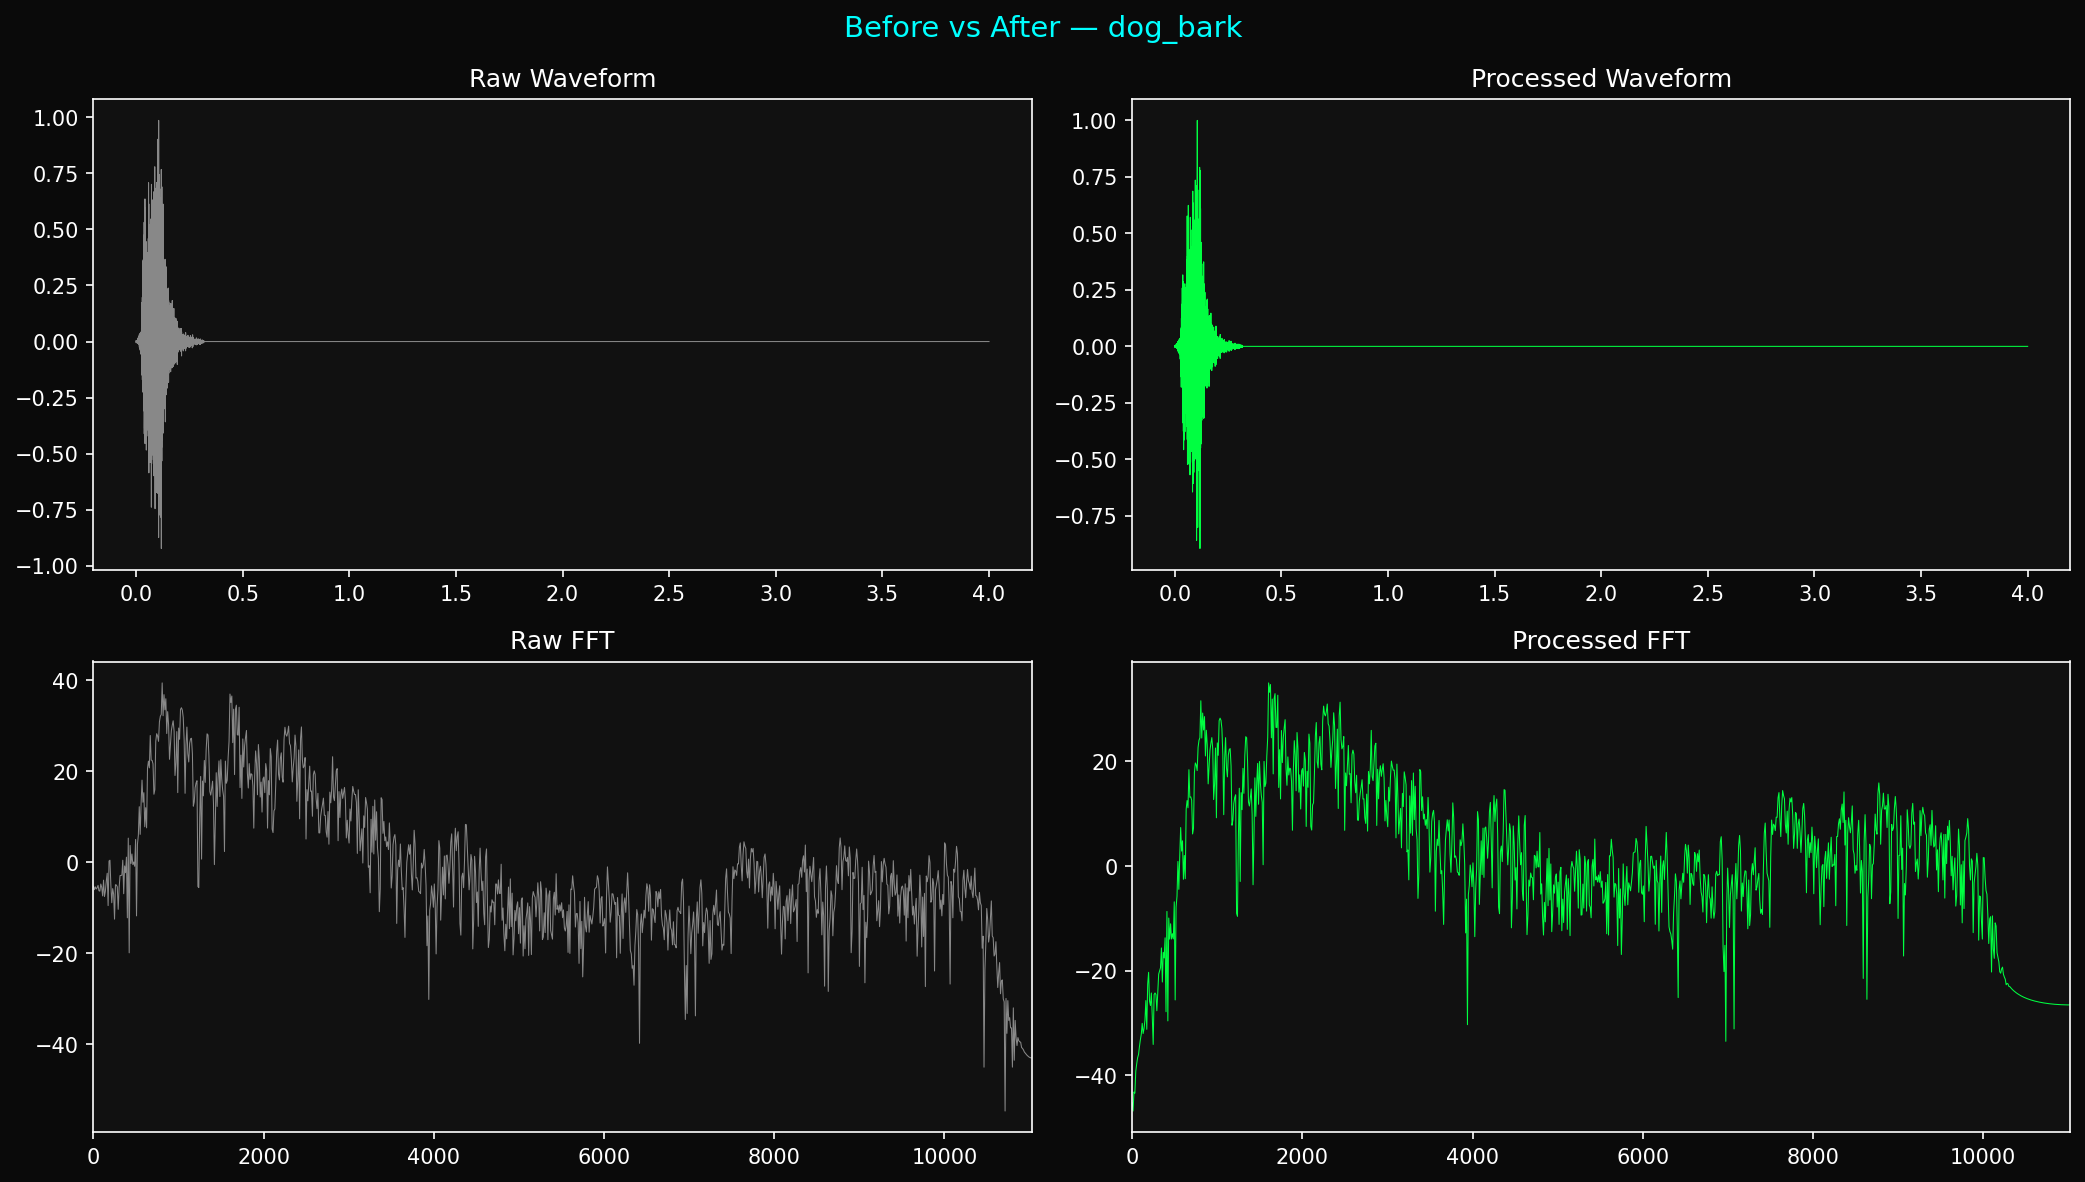
\includegraphics[width=\columnwidth]{fig_before_after_dog_bark.png}
    \caption{Example: before and after DSP preprocessing for \textit{dog\_bark} class (waveform and spectrogram).}
    \label{fig:before_after}
\end{figure}

% =============================================================================
\section{Feature Engineering}
\label{sec:features}

% -----------------------------------------------------------------------------
\subsection{Handcrafted Features (SVM \& Random Forest)}

A 931-dimensional feature vector is extracted from each audio clip, as detailed in \Cref{tab:features}. Seven summary statistics (mean, std, min, max, median, skewness, kurtosis) are computed for each per-frame feature over time.

\begin{table}[htbp]
\centering
\caption{Handcrafted feature vector composition (931 dimensions).}
\label{tab:features}
\begin{tabular}{@{}lrrr@{}}
\toprule
\textbf{Feature Group} & \textbf{Per-Frame} & \textbf{Stats} & \textbf{Dims} \\
\midrule
MFCC (40) + $\Delta$ + $\Delta\Delta$ & 120 & 7 & 840 \\
Spectral centroid       & 1   & 7 & 7 \\
Spectral bandwidth      & 1   & 7 & 7 \\
Spectral rolloff        & 1   & 7 & 7 \\
Spectral flatness       & 1   & 7 & 7 \\
Zero-crossing rate      & 1   & 7 & 7 \\
RMS energy              & 1   & 7 & 7 \\
Spectral contrast (7)   & 7   & 7 & 49 \\
\midrule
\textbf{Total}          &     &   & \textbf{931} \\
\bottomrule
\end{tabular}
\end{table}

% -----------------------------------------------------------------------------
\subsection{Mel Spectrogram (CNN-2D)}

For the CNN-2D model, mel spectrograms are extracted with the following parameters:
\begin{itemize}
    \item 128 mel bands, $f_{\min} = 50$~Hz, $f_{\max} = 10{,}000$~Hz
    \item FFT size: 2048, hop length: 512
    \item Output shape: $(128 \times 173)$ per clip
    \item Converted to log scale (dB), normalized per sample
\end{itemize}

\begin{figure}[htbp]
    \centering
    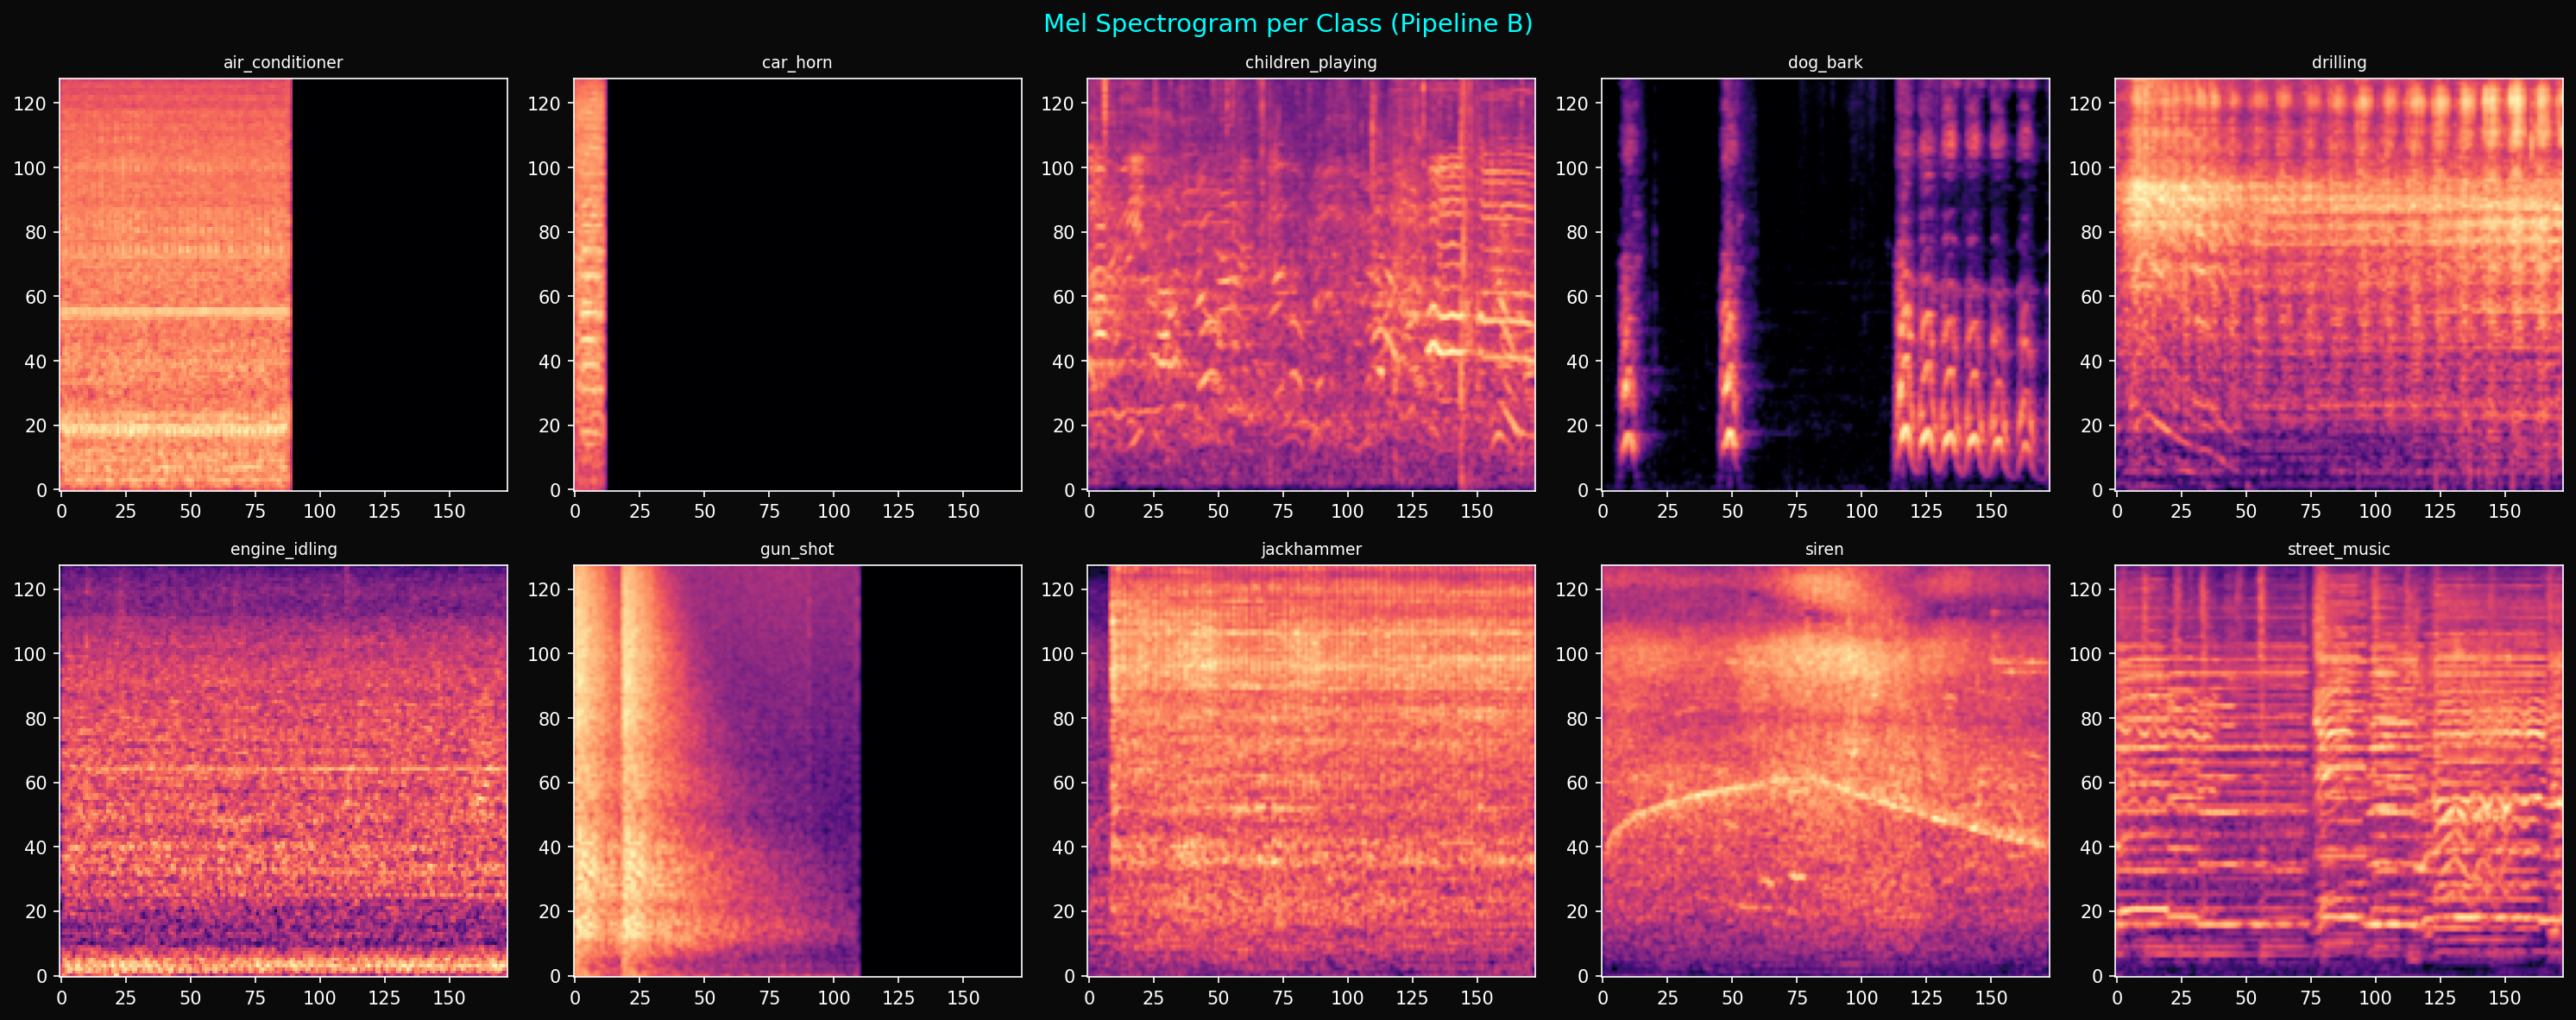
\includegraphics[width=\columnwidth]{fig_mel_spectrogram_per_class.png}
    \caption{Mel spectrogram examples for all 10 classes.}
    \label{fig:mel_specs}
\end{figure}

% -----------------------------------------------------------------------------
\subsection{Dimensionality Reduction}

For SVM, PCA reduces the feature space from 931 to 200 dimensions. This is necessary because SVM with RBF kernel has computational complexity $O(n^2 d)$, making 931 features prohibitively expensive for $\sim$7,800 training samples per fold.

Random Forest uses the full 931-dimensional vector, as tree-based methods handle high-dimensional data efficiently.

\begin{figure}[htbp]
    \centering
    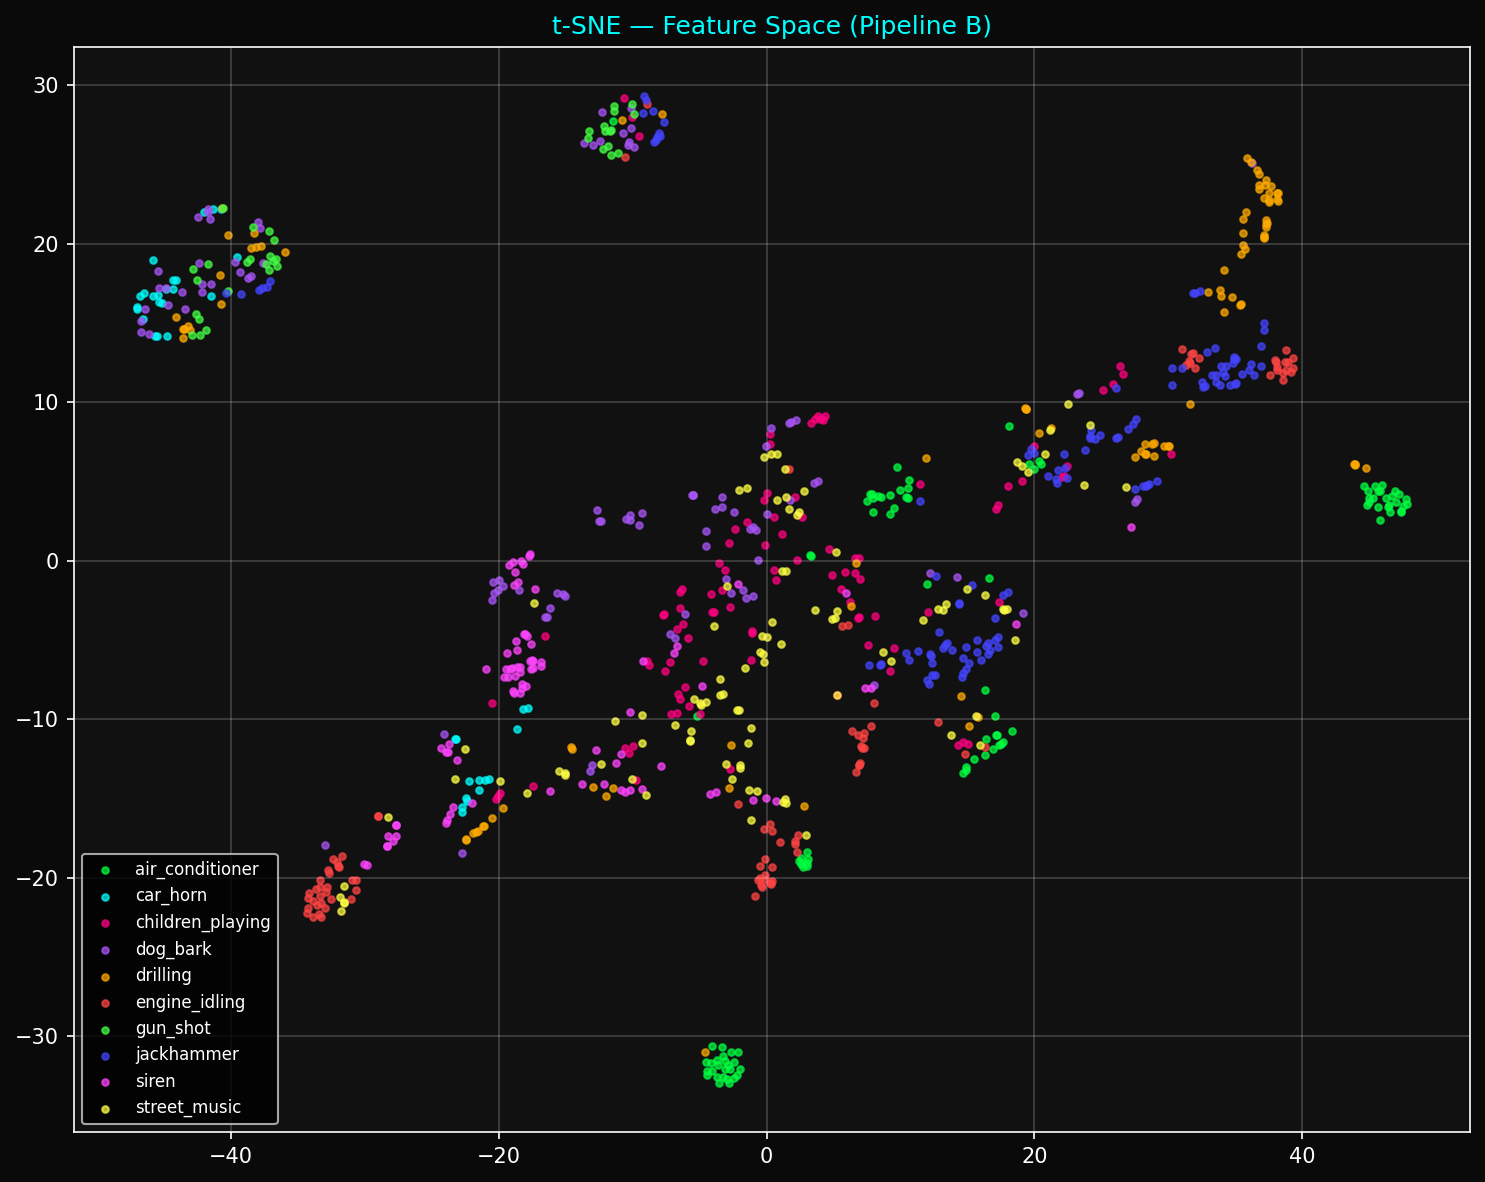
\includegraphics[width=\columnwidth]{fig_tsne_features.png}
    \caption{t-SNE visualization of the 931-dimensional feature space, showing class clustering patterns.}
    \label{fig:tsne}
\end{figure}

% =============================================================================
\section{Classification Models}
\label{sec:models}

% -----------------------------------------------------------------------------
\subsection{SVM (Support Vector Machine)}

\begin{itemize}
    \item Kernel: RBF (Radial Basis Function)
    \item Preprocessing: StandardScaler $\rightarrow$ PCA(200)
    \item Hyperparameters: $C = 10$, $\gamma = \text{scale}$
    \item Decision function:
\end{itemize}
\begin{equation}
    f(\mathbf{x}) = \text{sign}\left(\sum_i \alpha_i y_i K(\mathbf{x}_i, \mathbf{x}) + b\right)
    \label{eq:svm}
\end{equation}

% -----------------------------------------------------------------------------
\subsection{Random Forest}

\begin{itemize}
    \item 500 trees, unlimited depth
    \item Preprocessing: StandardScaler (no PCA)
    \item Full 931-dimensional feature vector
    \item Parallelized across all CPU cores
\end{itemize}

% -----------------------------------------------------------------------------
\subsection{CNN-2D (Convolutional Neural Network)}

The CNN architecture processes mel spectrograms of shape $(1 \times 128 \times 173)$ through four convolutional blocks followed by fully connected layers:

\begin{table}[htbp]
\centering
\caption{CNN-2D architecture.}
\label{tab:cnn}
\begin{tabular}{@{}ll@{}}
\toprule
\textbf{Layer} & \textbf{Output Shape} \\
\midrule
Input                            & $(1, 128, 173)$ \\
Conv2d$(1 \to 32, 3\times3)$ + BN + ReLU + MaxPool(2) & $(32, 63, 86)$ \\
Conv2d$(32 \to 64, 3\times3)$ + BN + ReLU + MaxPool(2) & $(64, 30, 42)$ \\
Conv2d$(64 \to 128, 3\times3)$ + BN + ReLU + MaxPool(2) & $(128, 14, 20)$ \\
Conv2d$(128 \to 256, 3\times3)$ + BN + ReLU + AdaptiveAvgPool(1) & $(256, 1, 1)$ \\
Flatten + Dropout(0.5)          & $(256)$ \\
Dense$(256 \to 128)$ + ReLU + Dropout(0.3) & $(128)$ \\
Dense$(128 \to 10)$             & $(10)$ \\
\bottomrule
\end{tabular}
\end{table}

\textbf{Training configuration:}
\begin{itemize}
    \item Optimizer: Adam ($\text{lr} = 0.001$)
    \item Loss: CrossEntropyLoss
    \item Scheduler: ReduceLROnPlateau (patience $= 3$, factor $= 0.5$)
    \item Early stopping: patience $= 5$ epochs
    \item Batch size: 64
    \item Device: Apple MPS (Metal Performance Shaders)
\end{itemize}

% =============================================================================
\section{Experimental Methodology}
\label{sec:methodology}

% -----------------------------------------------------------------------------
\subsection{Evaluation Protocol}

All experiments follow a strict 10-fold cross-validation scheme using \US{}'s predefined folds. Each fold serves as the test set once, with the remaining 9 folds for training. Folds are \textbf{never shuffled}---the same samples always remain in the same fold, as per dataset guidelines~\cite{salamon2014}.

% -----------------------------------------------------------------------------
\subsection{Metrics}

\begin{itemize}
    \item \textbf{Accuracy}: Fraction of correctly classified samples
    \item \textbf{F1 Score (macro)}: Harmonic mean of precision and recall, averaged across classes (handles class imbalance)
    \item \textbf{95\% Confidence Interval}:
\end{itemize}
\begin{equation}
    \text{CI} = 1.96 \cdot \frac{\sigma}{\sqrt{n}}, \quad n = 10 \text{ folds}
    \label{eq:ci}
\end{equation}

% -----------------------------------------------------------------------------
\subsection{Statistical Tests}

To determine whether the difference between \pipeA{} and \pipeB{} is statistically significant, three tests are applied:

\textbf{1. Paired $t$-test:} Tests if the mean per-fold difference is significantly different from zero.
\begin{equation}
    t = \frac{\bar{d}}{s_d / \sqrt{n}}, \quad \bar{d} = \frac{1}{n}\sum_{i=1}^{n}(a_i - b_i)
    \label{eq:ttest}
\end{equation}

\textbf{2. Wilcoxon signed-rank test:} Non-parametric alternative that does not assume normal distribution of differences.

\textbf{3. Cohen's $d$ (effect size):} Quantifies the magnitude of the difference.
\begin{equation}
    d = \frac{\bar{d}}{s_d}
    \label{eq:cohens_d}
\end{equation}

Interpretation: $|d| < 0.2$ = negligible, $0.2$--$0.5$ = small, $0.5$--$0.8$ = medium, $> 0.8$ = large.

% -----------------------------------------------------------------------------
\subsection{Feature Caching}

To avoid repeated feature extraction ($\sim$14 hours), all features were pre-extracted and cached: raw features ($8732 \times 931$), DSP features ($8732 \times 931$), raw mel spectrograms ($8732 \times 128 \times 173$), DSP mel spectrograms ($8732 \times 128 \times 173$), labels, and fold assignments.

% =============================================================================
\section{Results}
\label{sec:results}

% -----------------------------------------------------------------------------
\subsection{Classification Accuracy}

\Cref{tab:accuracy} presents the main accuracy results. Random Forest achieves the best overall performance (71.5\%), while CNN-2D shows the lowest accuracy (66.7\%) and highest variance.

\begin{table}[htbp]
\centering
\caption{Classification accuracy (\%) across 10 folds. Best model in bold.}
\label{tab:accuracy}
\begin{tabular}{@{}lcccc@{}}
\toprule
\textbf{Model} & \textbf{Pipe.\ A} & \textbf{Pipe.\ B} & $\boldsymbol{\Delta}$ & \textbf{$p$-value} \\
\midrule
SVM            & $70.1 \pm 3.2$ & $70.0 \pm 3.6$ & $-0.12$ & 0.846 \\
\textbf{Random Forest} & $\mathbf{71.5 \pm 2.6}$ & $71.2 \pm 2.2$ & $-0.26$ & 0.768 \\
CNN-2D         & $66.7 \pm 5.2$ & $67.6 \pm 4.8$ & $+0.94$ & 0.625 \\
\bottomrule
\end{tabular}
\end{table}

% -----------------------------------------------------------------------------
\subsection{F1 Score (Macro)}

\Cref{tab:f1} shows F1 scores, which account for class imbalance. The pattern mirrors accuracy results---no meaningful difference between pipelines.

\begin{table}[htbp]
\centering
\caption{Macro F1 Score (\%) across 10 folds.}
\label{tab:f1}
\begin{tabular}{@{}lcccc@{}}
\toprule
\textbf{Model} & \textbf{Pipe.\ A} & \textbf{Pipe.\ B} & $\boldsymbol{\Delta}$ & \textbf{$p$-value} \\
\midrule
SVM            & $71.2 \pm 3.1$ & $71.2 \pm 3.5$ & $-0.04$ & 0.955 \\
Random Forest  & $72.8 \pm 2.2$ & $72.6 \pm 1.9$ & $-0.21$ & 0.795 \\
CNN-2D         & $66.7 \pm 5.3$ & $66.8 \pm 5.3$ & $+0.08$ & 0.966 \\
\bottomrule
\end{tabular}
\end{table}

% -----------------------------------------------------------------------------
\subsection{Statistical Significance}

\Cref{tab:stats} summarizes the full statistical analysis. \textbf{None of the three models show a statistically significant difference} at the $\alpha = 0.05$ significance level.

\begin{table}[htbp]
\centering
\caption{Statistical significance tests for Pipeline~A vs.\ Pipeline~B.}
\label{tab:stats}
\begin{tabular}{@{}lcccc@{}}
\toprule
\textbf{Model} & \textbf{$t$-test $p$} & \textbf{Wilcoxon $p$} & \textbf{Cohen's $d$} & \textbf{Effect} \\
\midrule
SVM            & 0.846 & 0.557 & 0.063  & Negligible \\
Random Forest  & 0.768 & 0.846 & 0.096  & Negligible \\
CNN-2D         & 0.625 & 0.695 & $-0.160$ & Negligible \\
\bottomrule
\end{tabular}
\end{table}

% -----------------------------------------------------------------------------
\subsection{Per-Fold Analysis}

Per-fold accuracy shows high variance, particularly for CNN-2D (\Cref{fig:boxplot}):
\begin{itemize}
    \item SVM range: 63.4\%--78.6\% (Pipe.\ A), 62.8\%--78.6\% (Pipe.\ B)
    \item RF range: 62.7\%--78.5\% (Pipe.\ A), 65.9\%--78.0\% (Pipe.\ B)
    \item CNN range: 53.6\%--78.0\% (Pipe.\ A), 54.6\%--81.1\% (Pipe.\ B)
\end{itemize}

\begin{figure}[htbp]
    \centering
    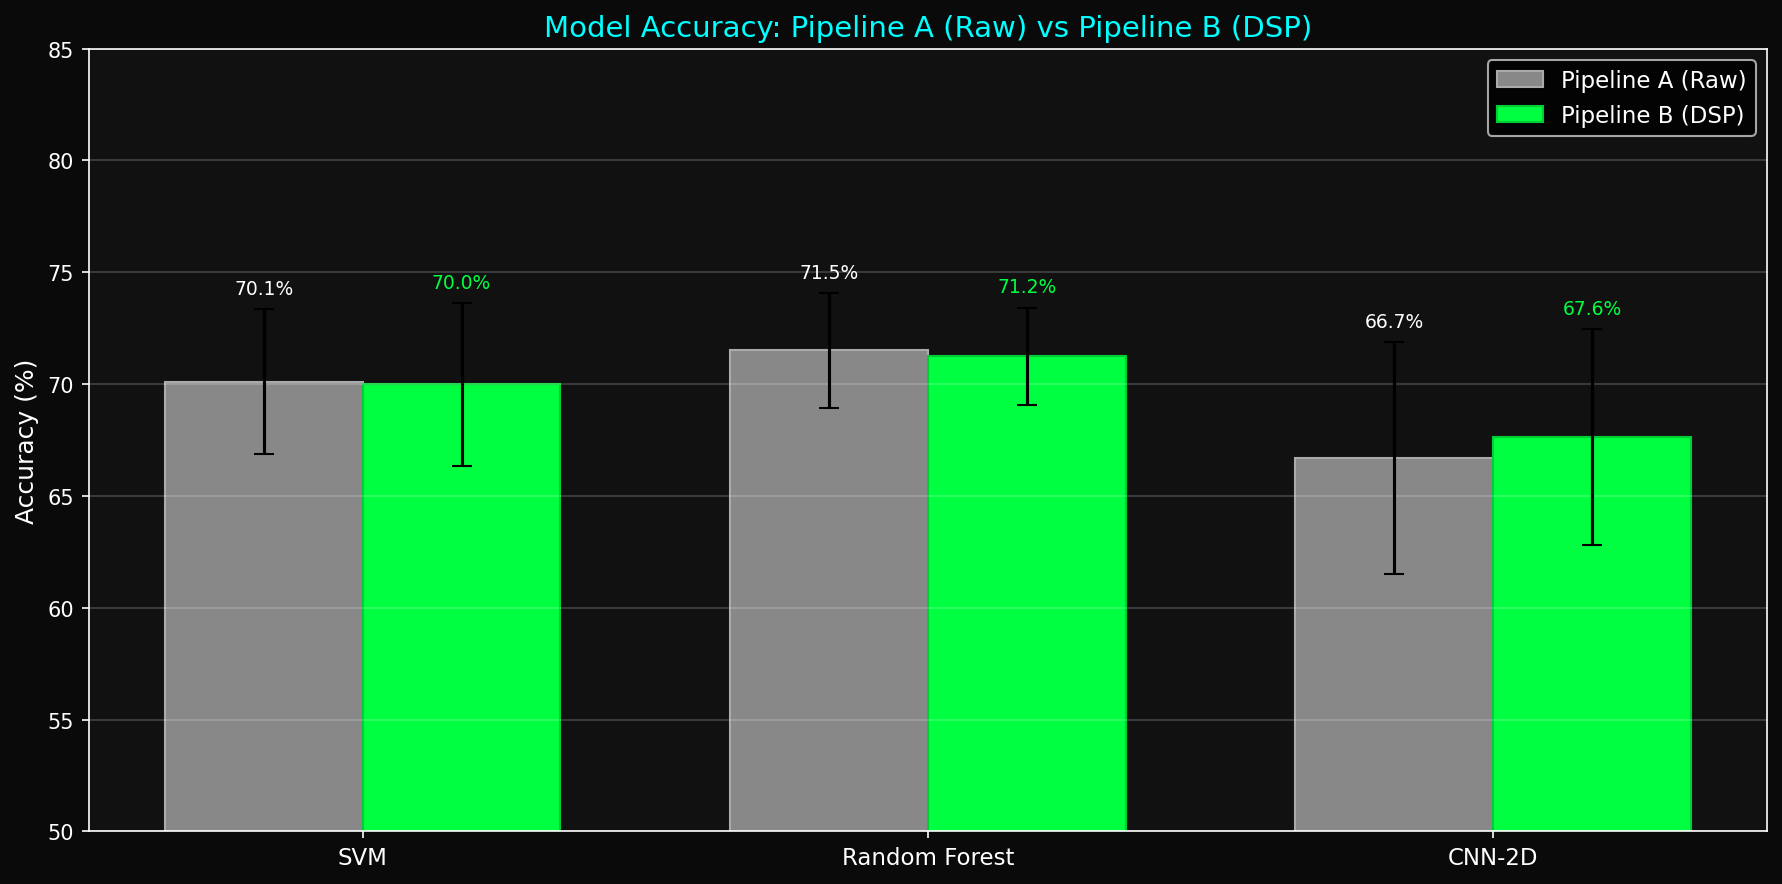
\includegraphics[width=\columnwidth]{fig_accuracy_comparison_barplot.png}
    \caption{Pipeline~A vs.\ Pipeline~B accuracy comparison across models.}
    \label{fig:accuracy_bar}
\end{figure}

\begin{figure}[htbp]
    \centering
    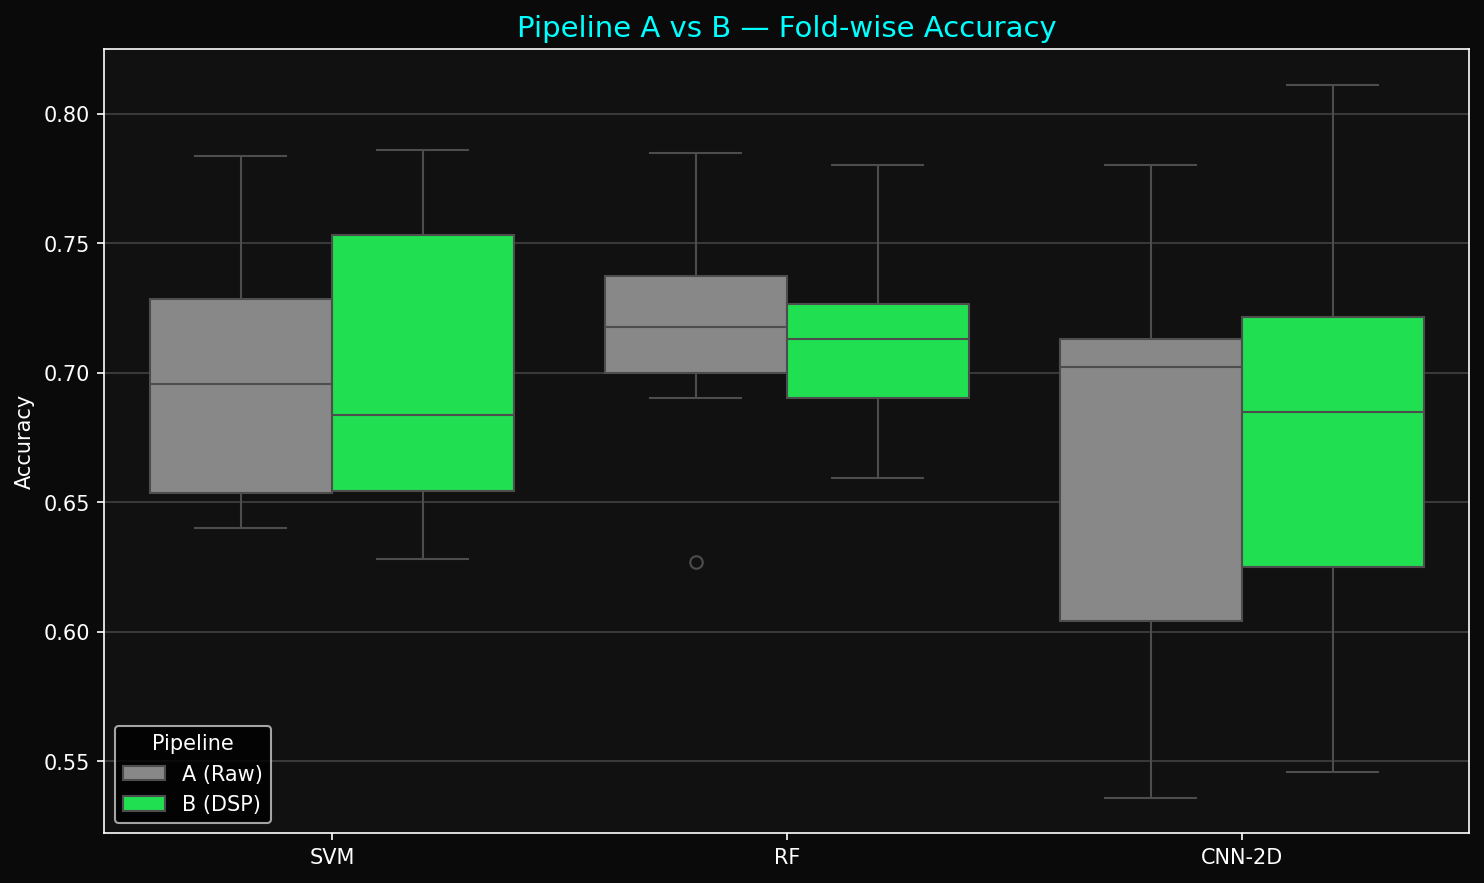
\includegraphics[width=\columnwidth]{fig_fold_accuracy_boxplot.png}
    \caption{Box plot of per-fold accuracy distribution for all models and pipelines.}
    \label{fig:boxplot}
\end{figure}

\begin{figure}[htbp]
    \centering
    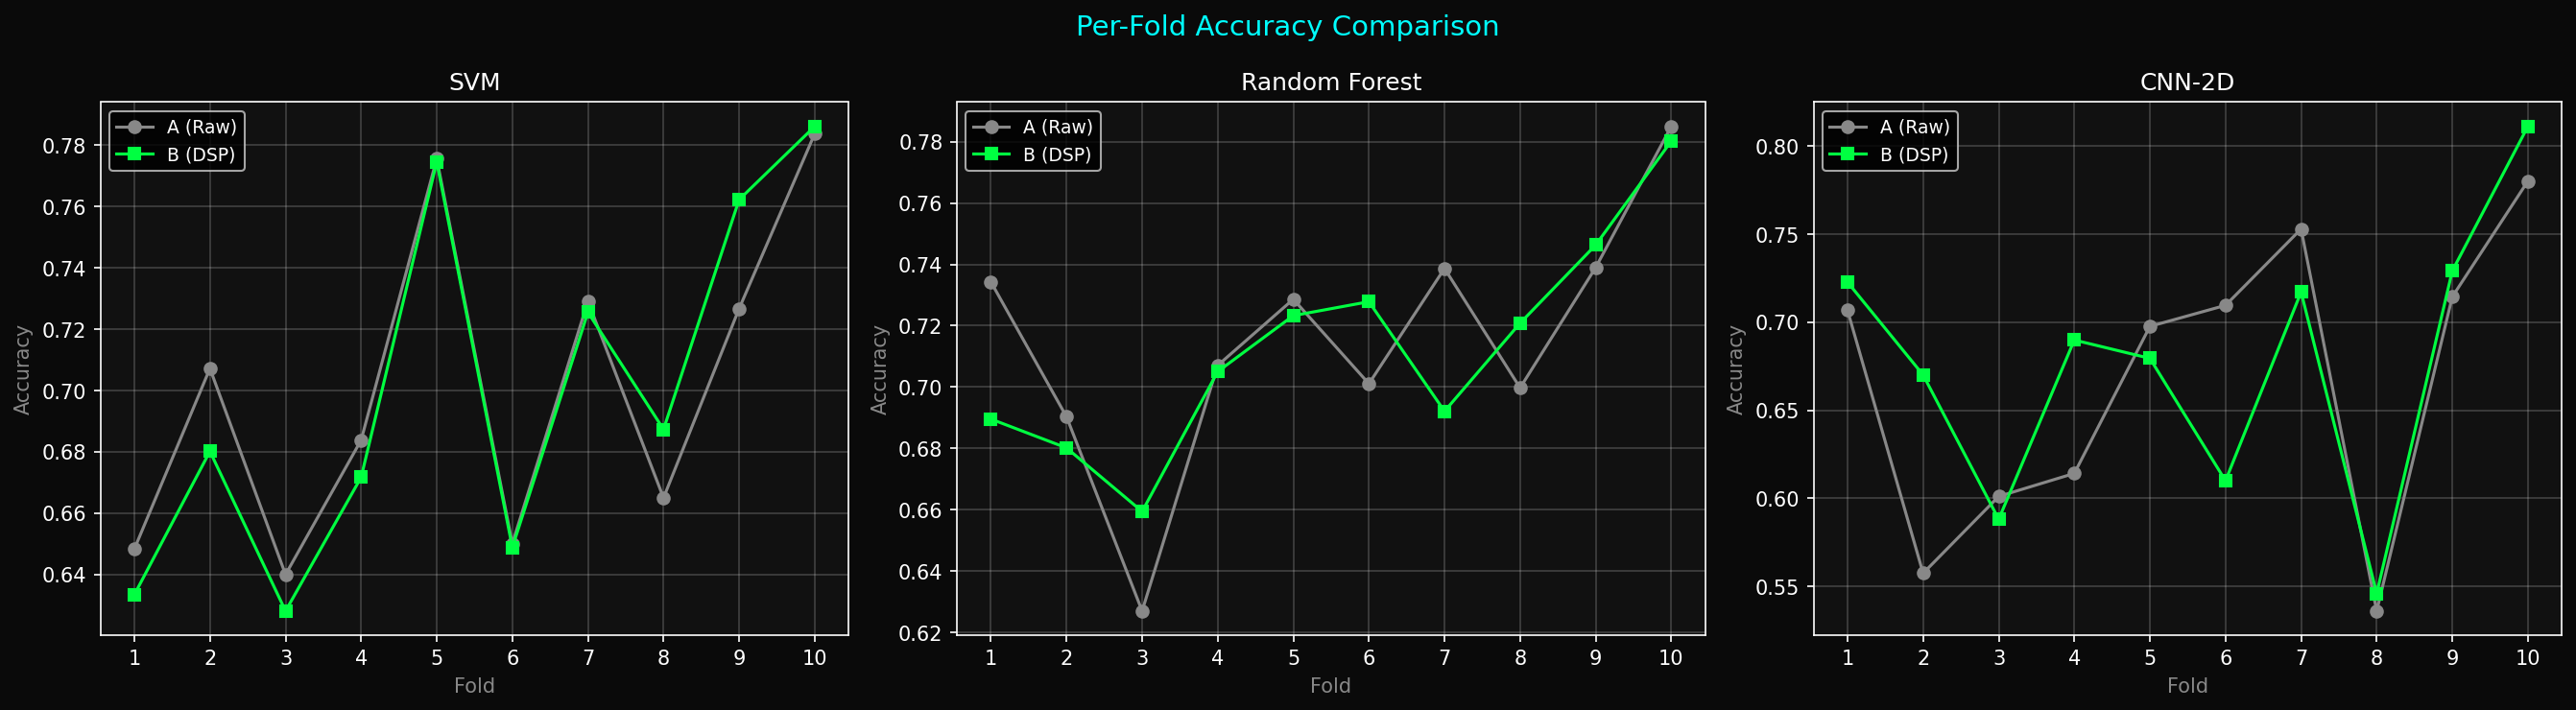
\includegraphics[width=\columnwidth]{fig_per_fold_accuracy.png}
    \caption{Per-fold accuracy line plots for all models.}
    \label{fig:per_fold}
\end{figure}

% =============================================================================
\section{Analysis and Discussion}
\label{sec:discussion}

% -----------------------------------------------------------------------------
\subsection{Why Doesn't DSP Help?}

The central finding---that explicit DSP preprocessing provides no significant improvement---can be explained by the \textbf{redundancy between DSP preprocessing and modern feature extraction}:

\begin{enumerate}
    \item \textbf{MFCC computation} applies mel-scale filterbanks (effectively bandpass filtering) and computes cepstral coefficients, already emphasizing perceptually relevant frequency bands.

    \item \textbf{Mel spectrogram parameters} use $f_{\min} = 50$~Hz and $f_{\max} = 10{,}000$~Hz---the \textit{same passband} as our FIR filter. The mel spectrogram inherently ignores frequencies outside this range.

    \item \textbf{Statistical aggregation} (mean, std, skewness, kurtosis over time frames) provides robustness against noise, similar to what filtering aims to achieve.

    \item \textbf{StandardScaler} in the ML pipeline normalizes features to zero mean and unit variance, overlapping with the effect of amplitude normalization.
\end{enumerate}

In essence, the feature extraction stage already captures what DSP preprocessing aims to provide, making the explicit DSP step redundant.

% -----------------------------------------------------------------------------
\subsection{Model Comparison}

\begin{itemize}
    \item \textbf{Random Forest} achieves the best results (71.5\%), benefiting from its ability to handle 931 dimensions without PCA and providing interpretable feature importance (\Cref{fig:importance}).
    \item \textbf{SVM} achieves comparable results (70.1\%) but required PCA reduction to 200 dimensions for computational feasibility.
    \item \textbf{CNN-2D} underperforms classical ML (66.7\%), likely due to the limited dataset size ($\sim$7,800 training samples per fold).
\end{itemize}

\begin{figure}[htbp]
    \centering
    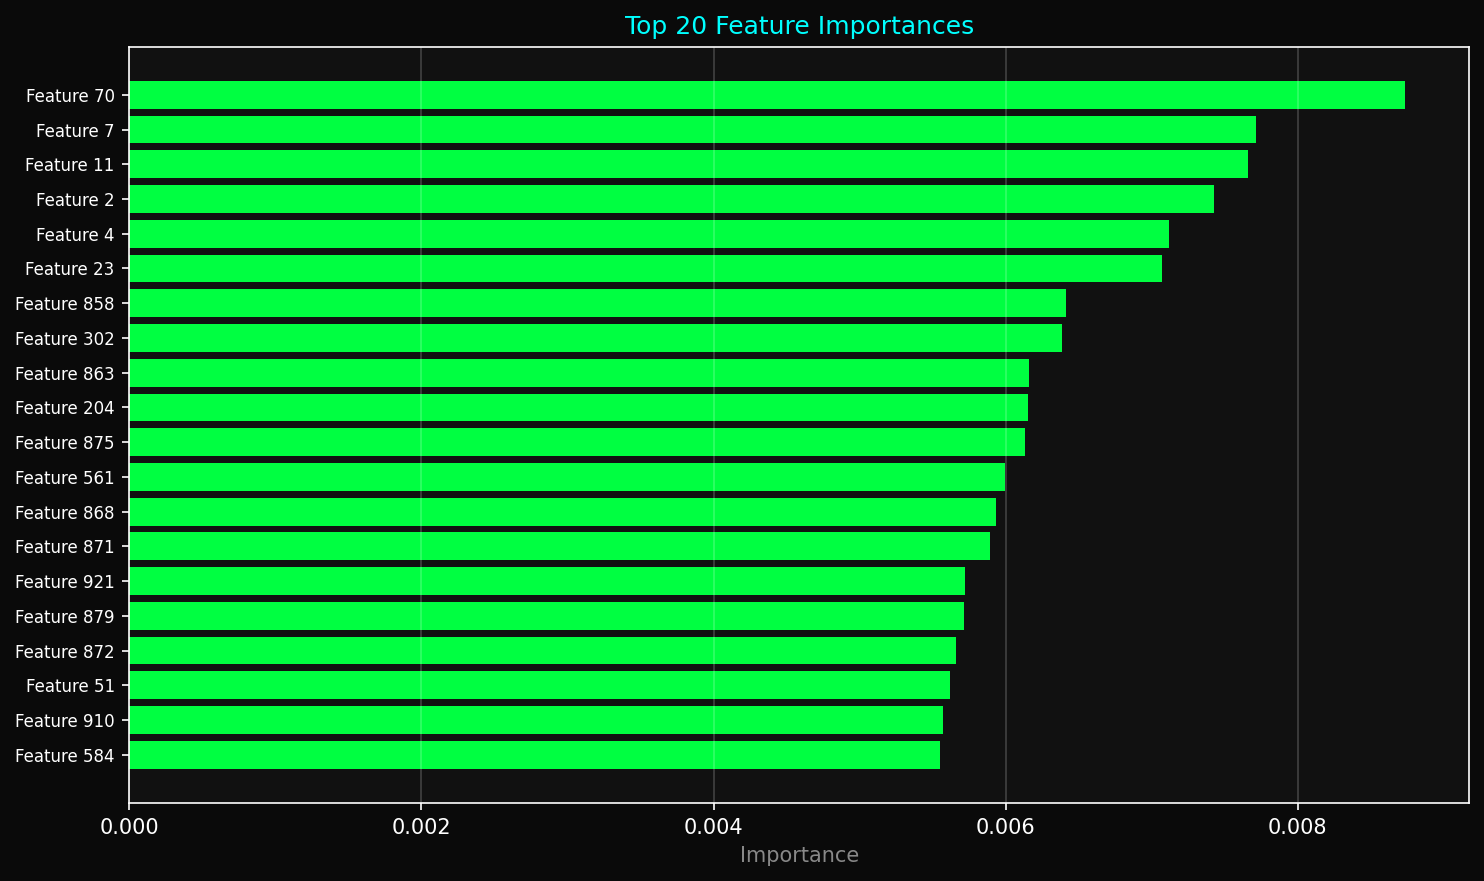
\includegraphics[width=\columnwidth]{fig_feature_importance.png}
    \caption{Random Forest feature importance, showing which features contribute most to classification.}
    \label{fig:importance}
\end{figure}

% -----------------------------------------------------------------------------
\subsection{CNN Performance Analysis}

The CNN-2D exhibits the highest fold-to-fold variance ($\text{CI} = 5.2\%$) and lower absolute accuracy than classical ML. This is expected for deep learning on small datasets:
\begin{itemize}
    \item $\sim$7,800 training samples is relatively small for a 4-layer CNN
    \item Early stopping (patience $= 5$) may prevent full convergence on some folds
    \item Data augmentation (not implemented) could significantly improve CNN performance
\end{itemize}

% -----------------------------------------------------------------------------
\subsection{Limitations}

\begin{enumerate}
    \item \textbf{No data augmentation}: CNN performance could improve with time-shifting, pitch-shifting, and noise injection
    \item \textbf{Fixed SVM hyperparameters}: Exhaustive grid search was limited for computational reasons; optimal $C$/$\gamma$ could improve SVM results
    \item \textbf{No per-class analysis}: Some classes may benefit from DSP more than others
    \item \textbf{Single filter configuration}: Only one FIR design (50--10,000~Hz, order 101) was tested; different passbands might yield different results
    \item \textbf{No pre-trained models}: Transfer learning from large audio models (e.g., VGGish, PANNs) was not explored
\end{enumerate}

% =============================================================================
\section{Conclusion}
\label{sec:conclusion}

% -----------------------------------------------------------------------------
\subsection{Answer to Research Question}

\textbf{DSP preprocessing does not significantly improve environmental sound classification accuracy.} Across all three models (SVM, Random Forest, CNN-2D), the differences between \pipeA{} (raw) and \pipeB{} (DSP-preprocessed) are:
\begin{itemize}
    \item Not statistically significant (all $p > 0.05$)
    \item Negligible in effect size (all $|d| < 0.2$)
    \item Practically insignificant ($|\Delta| < 1\%$)
\end{itemize}

% -----------------------------------------------------------------------------
\subsection{Key Takeaways}

\begin{enumerate}
    \item Modern feature extraction (MFCCs, mel spectrograms) already implicitly performs the filtering and normalization that explicit DSP preprocessing provides.

    \item Classical ML (Random Forest: 71.5\%) outperforms deep learning (CNN-2D: 66.7\%) on this dataset size ($\sim$8,700 samples).

    \item The FIR bandpass filter does improve raw signal SNR ($+2.9$ to $+4.5$~dB for some classes), but this improvement does not translate to better classification accuracy.

    \item DSP preprocessing is not wasted---understanding filter design, frequency analysis, and signal characteristics provides valuable engineering insight even when the classification improvement is negligible.
\end{enumerate}

% -----------------------------------------------------------------------------
\subsection{Future Work}

\begin{itemize}
    \item Apply data augmentation for CNN training (time-shift, pitch-shift, noise injection)
    \item Test class-specific DSP preprocessing (e.g., different filters for stationary vs.\ non-stationary sounds)
    \item Experiment with deeper architectures or pre-trained models (VGGish, PANNs)
    \item Investigate attention mechanisms for variable-length audio
    \item Evaluate on larger datasets (ESC-50, AudioSet) to test generalizability
\end{itemize}

% =============================================================================
\section*{Acknowledgments}

This project uses the UrbanSound8K dataset provided by Salamon et al.~\cite{salamon2014} via the Urban Sound Taxonomy project at New York University.

% =============================================================================
\bibliographystyle{IEEEtran}

\begin{thebibliography}{4}

\bibitem{salamon2014}
J.~Salamon, C.~Jacoby, and J.~P.~Bello, ``A dataset and taxonomy for urban sound research,'' in \textit{Proc.\ 22nd ACM Int.\ Conf.\ Multimedia}, 2014, pp.~1041--1044.

\bibitem{oppenheim2010}
A.~V.~Oppenheim and R.~W.~Schafer, \textit{Discrete-Time Signal Processing}, 3rd~ed.\hskip 1em Pearson, 2010.

\bibitem{davis1980}
S.~Davis and P.~Mermelstein, ``Comparison of parametric representations for monosyllabic word recognition in continuously spoken sentences,'' \textit{IEEE Trans.\ Acoust., Speech, Signal Process.}, vol.~28, no.~4, pp.~357--366, 1980.

\bibitem{piczak2015}
K.~J.~Piczak, ``Environmental sound classification with convolutional neural networks,'' in \textit{Proc.\ IEEE 25th Int.\ Workshop Mach.\ Learn.\ Signal Process.\ (MLSP)}, 2015, pp.~1--6.

\end{thebibliography}

% =============================================================================
\appendix

\section{Reproducibility}
\label{app:reproducibility}

\subsection{Environment}
\begin{itemize}
    \item Python 3.13.2
    \item PyTorch 2.6 (MPS backend for macOS)
    \item scikit-learn 1.6
    \item librosa 0.10
    \item scipy 1.15
\end{itemize}

\subsection{Random Seeds}
All experiments use \texttt{RANDOM\_SEED = 42}. NumPy, PyTorch, and scikit-learn seeds are set before each fold for full reproducibility.

\subsection{Data Processing}
UrbanSound8K v2 from Zenodo. 10 predefined folds, never shuffled. Audio resampled to 22,050~Hz, padded/truncated to 4~seconds (88,200 samples).

\subsection{Code}
All source code is available in the \texttt{src/} directory. Jupyter notebooks in \texttt{notebooks/} reproduce the full pipeline from raw data to final results. Run notebooks sequentially: \texttt{01} $\rightarrow$ \texttt{02} $\rightarrow$ \texttt{03} $\rightarrow$ \texttt{04} $\rightarrow$ \texttt{05} $\rightarrow$ \texttt{06}.

\subsection{All Hyperparameters}
\begin{table}[H]
\centering
\caption{Complete hyperparameter configuration.}
\label{tab:hyperparams}
\begin{tabular}{@{}ll@{}}
\toprule
\textbf{Parameter} & \textbf{Value} \\
\midrule
\multicolumn{2}{@{}l}{\textit{Audio}} \\
\quad Sample rate & 22,050~Hz \\
\quad Duration & 4~s (88,200 samples) \\
\midrule
\multicolumn{2}{@{}l}{\textit{DSP}} \\
\quad FIR passband & 50--10,000~Hz \\
\quad FIR order & 101 taps \\
\quad IIR order & 5 (Butterworth) \\
\quad Pre-emphasis $\alpha$ & 0.97 \\
\midrule
\multicolumn{2}{@{}l}{\textit{Features}} \\
\quad MFCC coefficients & 40 \\
\quad Mel bands & 128 \\
\quad FFT size & 2048 \\
\quad Hop length & 512 \\
\midrule
\multicolumn{2}{@{}l}{\textit{SVM}} \\
\quad Kernel & RBF \\
\quad $C$ & 10 \\
\quad $\gamma$ & scale \\
\quad PCA components & 200 \\
\midrule
\multicolumn{2}{@{}l}{\textit{Random Forest}} \\
\quad Trees & 500 \\
\quad Max depth & None (unlimited) \\
\midrule
\multicolumn{2}{@{}l}{\textit{CNN-2D}} \\
\quad Epochs & 100 (early stop) \\
\quad Batch size & 64 \\
\quad Learning rate & 0.001 \\
\quad Patience & 5 \\
\bottomrule
\end{tabular}
\end{table}

\balance
\end{document}
